\documentclass{article}
\usepackage{graphicx}
\usepackage{url}

%% http://www.ctan.org/tex-archive/help/Catalogue/entries/igo.html
\usepackage{igo}
\gobansize{9}

\usepackage[empty,cm]{fullpage}
\begin{document}

%% The first page includes a 9x9 board.
\centerline{\Huge WPI Go Beginner's Night}
\centerline{\Huge 7pm Friday, February 20, 2009}
\centerline{\Huge @ Campus Center, 2nd floor}
\vfill

\begin{center}
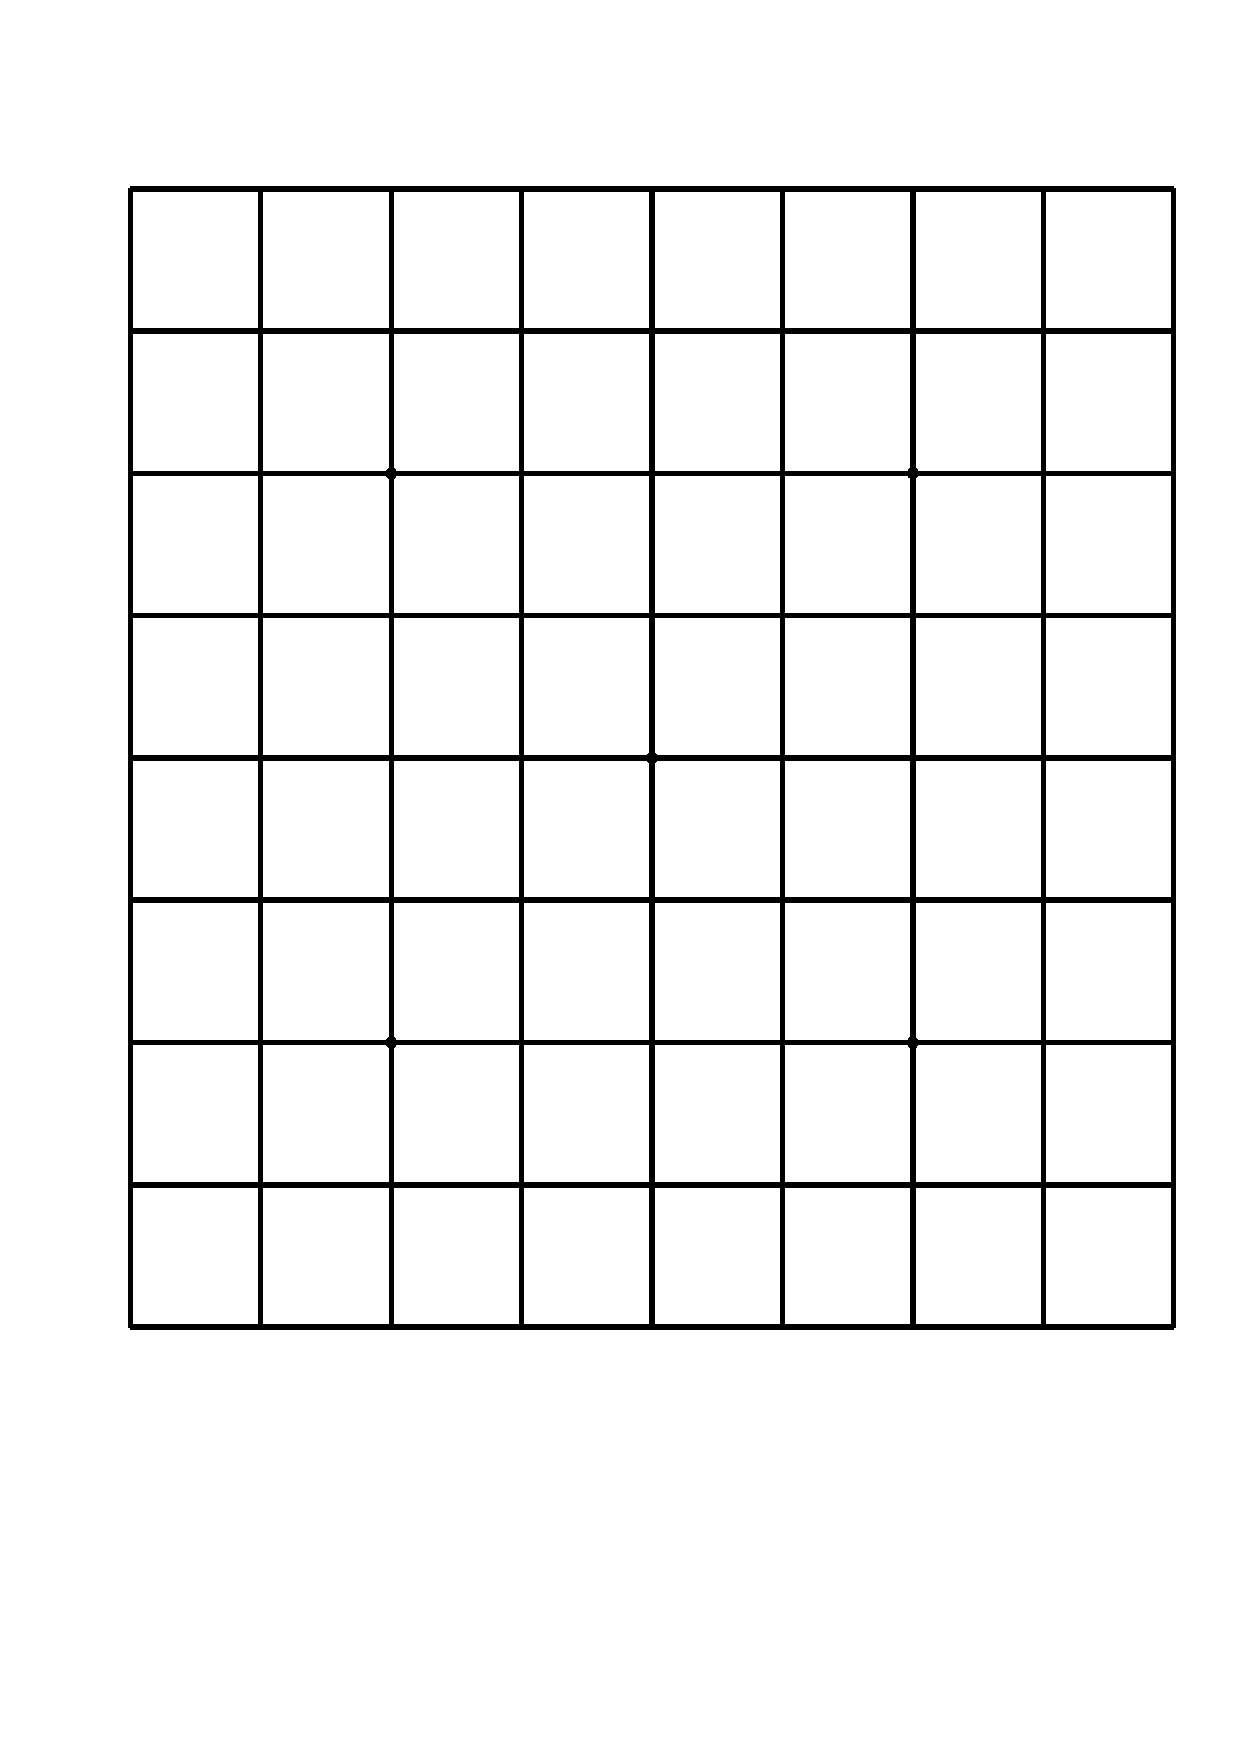
\includegraphics{gb9.epsi}
\end{center}

\vfill

\newpage

%% The next page includes a small description of the capturing rules,
%% a few puzzles, and references for more information.
\section*{Introduction}
Go is a board game between Black and White; the two take turns playing
on the intersections of the board.  The board starts out empty, and
the goal is not necessarily to capture the opponent's stone pieces, but to
take majority control over the board.  That being said, control of the
board is intimately related to capture, so let's show how to capture
stones.

Adjacent stones of the same color form a \emph{group} that lives or
dies as one.  (Diagonals don't count!)

\begin{center}
\cleargoban
\gobansize{19}
\shortstack{
\black{a1,a2,b3,c3,d3,d2}
\showgoban\\Two Black groups.}
\hspace{.5in}%
\shortstack{
\cleargoban
\white{d6,d5,d4,e4,f4,f5,f6,d6,e6}
\showgoban\\One White group.}
\hspace{.5in}%
\shortstack{
\cleargoban
\black{d9,d10,e8,f9,g8,h9,h10}
\white{k10,l10,m10,n10,o10,l9,l8,n9,n8}
\showgoban\\Five Black groups and one White group.}
\end{center}
%
A group stays on the board as long as it's adjacent to a vacant
intersection.  But if the opposing player places a stone that occupies
the last empty space of a group, that group is captured and removed
from the board.


\begin{center}
\shortstack{
\cleargoban
\black{a1,a2,b3,c3,d3,d2}
\white{a3,a4,b4,c4,d4,e4,e3,e2,e1,d1,c1,c2,b1}
\showgoban
\hspace{.2in}
\white[\igotriangle]{b2}
\showgoban
\hspace{.2in}
\cleargoban
\white{a3,a4,b4,c4,d4,e4,e3,e2,e1,d1,c1,c2,b1,b2}
%
\showgoban\\Figure~1: White's play at \whitestone[\igotriangle] will capture
both black groups.}
\end{center}


\begin{center}
%
\shortstack{
\cleargoban
\white{d6,d5,d4,e4,f4,f5,f6,d6,e6}
\black{c6,c5,c4,d3,e3,f3,g4,g5,g6,d7,e7,f7}
\showgoban
\hspace{.2in}
\black[\igotriangle]{e5}
\showgoban
\hspace{.2in}
\cleargoban
\black{c6,c5,c4,d3,e3,f3,g4,g5,g6,d7,e7,f7,e5}
\showgoban
\\
Figure~2: Black's play at \blackstone[\igotriangle] will capture the white group.}
\end{center}
Suicidal plays are disallowed, except for the special case where the
play is a capturing one, as in Figure~2.



%\section*{Puzzles}
%\begin{center}
%\cleargoban
%\shortstack{
%\black{}
%\showgoban\\Where can black play to capture a white group?}
%\hspace{1in}%
%\shortstack{
%\cleargoban
%\black{}
%\showgoban\\Where can black play to capture a white group?}
%\hspace{1in}%
%\shortstack{
%\cleargoban
%\black{}
%\showgoban\\Where can white play to capture a white group?
%\\(Warning: this is a trick question.)}
%\end{center}




%% Game taken from http://www.societies.cam.ac.uk/cugos/go/rules_06.html
\section*{A 9x9 game}
To help give a quick (but incomplete!) impression, here's an example
of a 9x9 game.
%
\begin{center}
\shortstack{
\gobansize{9}
\cleargoban
\black[1]{d7,f4,c4,f7,f6,g6,f5,g5,g7,f8}
\showfullgoban\\Moves 1--10.}
\hspace{1in}%
\shortstack{
\cleargobansymbols
\black[11]{e7,g8,e4,f3,e3,e2,d2,f2,c3,c9}
\showfullgoban\\Moves 11--20.}
\hspace{1in}%
\shortstack{
\cleargobansymbols
\black[21]{c8,e9,b9,d9,b7,e8,e1,f1,d1,d8}
\showfullgoban\\Moves 21--30.}
\end{center}
%
Black and White jostle and push against each other.  Black emphasizes
the left side of the board, and White the right side.  We'll talk
about how to evaluate the score in a future handout.  But as a teaser:
at the end of the game, Black gets 27 points, and White gets 26
points, so Black wins.


\section*{For more information...}
\begin{itemize}
\item \emph{WPI Go} (\url{http://go.hashcollision.org/}) is our homepage.

\item \emph{Sensei's Library} (\url{http://senseis.xmp.net/}), a wiki
  devoted to the game.

\item \emph{The Interactive Way to Go}
  (\url{http://playgo.to/interactive/}), which gives a more leisurely
  introduction.

\item Come to the Beginner's Night!  7pm on Friday, February 20, in
  the Campus Center.  We'll be on the second floor.
\end{itemize}
\end{document}
